% --- SEZIONE 3: ARCHITETTURE E COMPILAZIONE ---
\section{Adressierungsarten ARM (Cortex-M0)}\vspace{-1em}

\begin{minipage}[t]{0.49\columnwidth}
    \subsection{Register Direkt, Immediate}
    \begin{itemize}
        \item \textbf{Immediate:} \texttt{MOV R0, \#100} $\rightarrow$ Valore caricato direttamente.
        \item \textbf{Register:} \texttt{MOVS R2, R1} $\rightarrow$ Copia valore tra registri.
        \item \textbf{Limitazioni:} Gli immediati sono codificati nell'istruzione (es. 8-bit per \texttt{MOVS}).
    \end{itemize}

    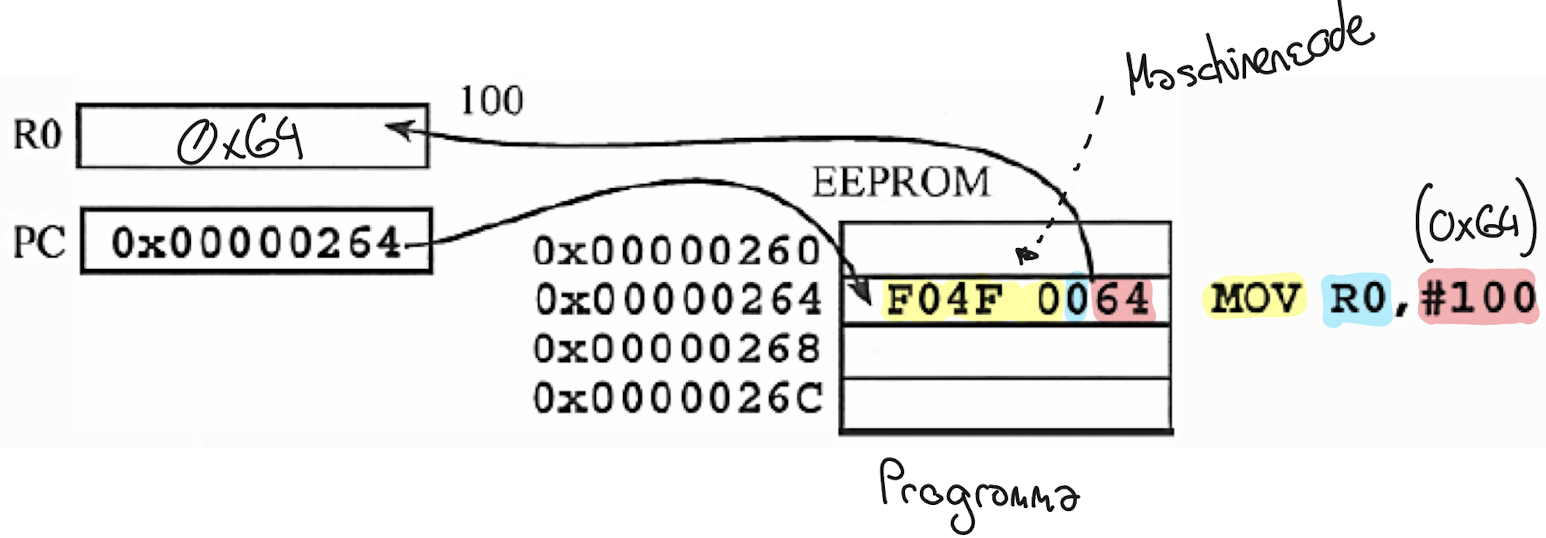
\includegraphics[width=\linewidth]{images/register_direkt.png}
\end{minipage}
\begin{minipage}[t]{0.5\columnwidth}
    \subsection{Register Indirekt (ptr)}
    \begin{itemize}
        \item \textbf{Semplice:} \texttt{LDR R0, [R1]} \\
        $\rightarrow$ $R0 = \text{valore all'indirizzo } R1$.
        \item \textbf{Con Offset:} \texttt{LDR R0, [R1, \#4]} $\rightarrow$ $R0 = \text{valore all'indirizzo } R1 + 4$ (utile per array/struct).
        \item \textbf{Con Index:} \texttt{LDR R0, [R1, R2]} \\
        $\rightarrow$ $R0 = \text{valore all'indirizzo } R1 + R2$.
    \end{itemize}    
    \begin{center}
        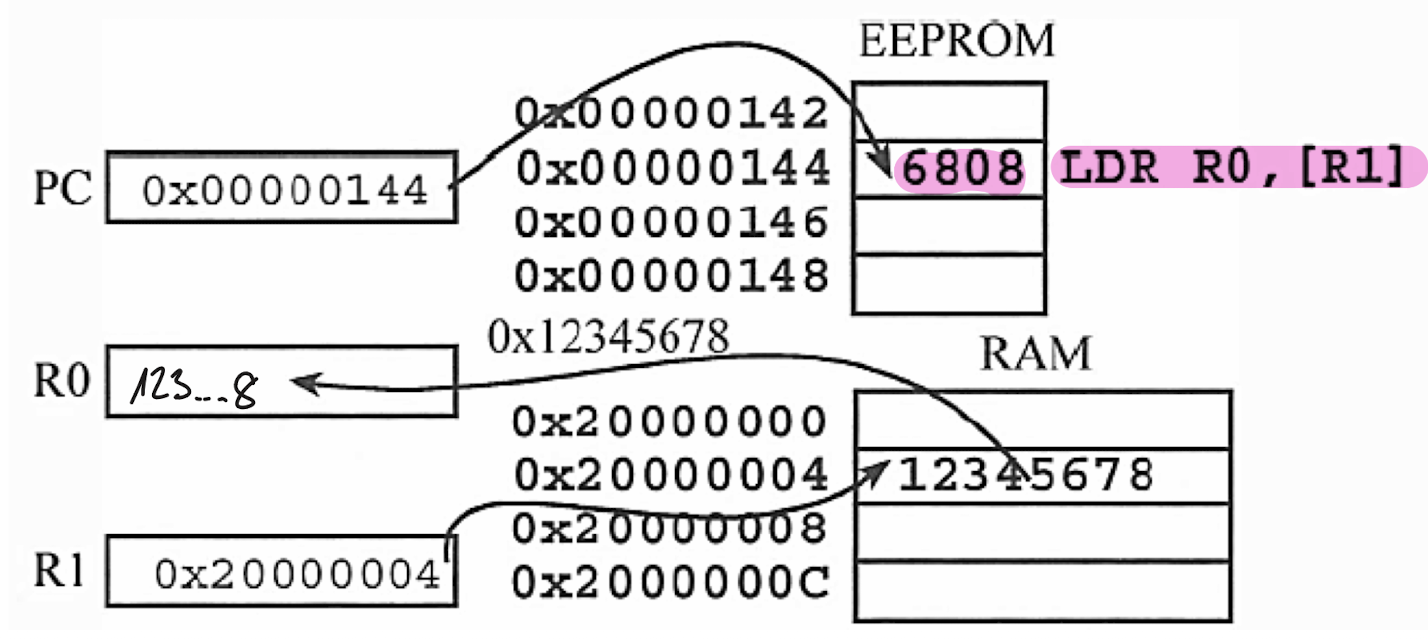
\includegraphics[width=\linewidth]{images/register_indirekt.png}
    \end{center}
\end{minipage}

\subsection{PC-Relative \& Literal Pool}
\begin{itemize}
    \item \textbf{Problema:} Istruzioni da 32-bit non possono contenere costanti da 32-bit.
    \item \textbf{Soluzione:} L'assembler salva la costante nel \textbf{Literal Pool} (zona memoria vicina).
    \item \textbf{Accesso:} \texttt{LDR R0, =0x12345678} viene tradotto in \texttt{LDR R0, [PC, \#offset]}.
    \item Richiedono sempre \textbf{due accessi} alla memoria
\end{itemize}

\subsection{Registerlisten \& Stack (SP-Relative)}
\begin{itemize}
    \item \textbf{Multiple:} \texttt{LDM R7!, \{R0-R3, R5\}} $\rightarrow$ Carica più registri partendo da indirizzo in $R7$.
    \item \textbf{Stack:} \texttt{PUSH \{R0-R2\}}, \texttt{POP \{R0-R2\}}.
    \item \textbf{Regola d'oro:} Il registro con numero più basso (\texttt{R0}) va sempre all'indirizzo di memoria più basso. L'ordine nelle graffe non conta per l'hardware.
\end{itemize}

\subsection{Stack Framing}
Lo Stack Frame è lo spazio riservato nella RAM per le variabili locali di una funzione.

\begin{itemize}
    \item \textbf{Allocazione:} \texttt{SUB SP, SP, \#X} riserva $X$ byte (lo stack cresce verso indirizzi bassi).
    \item \textbf{Frame Pointer ($R7$):} \texttt{MOV R7, SP} per avere un riferimento fisso all'inizio del frame.
    \item \textbf{Accesso:} var. vengono scritte/lette usando offset rispetto a $R7$, es: \texttt{STR R0, [R7, \#4]}.
    \item \textbf{Deallocazione:} Prima del ritorno (\texttt{BX LR}), si deve pulire lo stack con \texttt{ADD SP, SP, \#X}.
\end{itemize}